\documentclass{memoir}
\usepackage{graphicx}
\usepackage{amsmath}
\usepackage{float}
\usepackage[english]{babel}
\usepackage[english = american]{csquotes}
\MakeOuterQuote{"}
\usepackage[pdfpagemode=useNone,pdfstartview=FitH,colorlinks=true,linkcolor=blue,citecolor=blue,urlcolor=blue]{hyperref}
\usepackage[all]{hypcap}
\title{General Relativity Explained}
\author{physicsnerd}
\addtopsmarks{headings}{}{
\createmark{chapter}{both}{nonumber}{}{}
}

\begin{document}
\frontmatter
\maketitle
\tableofcontents
\chapter{Preface}
How can we shape society through revolution? It is an important question.

Einstein published the theory of special relativity in 1905 and the theory of general relativity in 1915. 
That marked an incredible revolution in both physics and modern thought. 
While most don’t even know how general relativity works on an intuitive level, let alone a mathematical level, 
the theory has transformed philosophy, showing that there must have been some beginning to the universe 
(the current theory of which is the Big Bang). 
People have been confronted with a result that contradicts their religion (or lack of one) or confirms it. 
Further, general relativity resulted in the discovery of black holes and more recently gravitational waves. 
These discoveries put both physicists and non-physicists alike in awe of the universe and the mysteries it holds. 
Finally, it has resulted in the biggest conflict in science perhaps ever: the conflict between general relativity and quantum mechanics. 
Scientists still are struggling (though they have made significant process) to figure out a correct theory 
that explains the universe as we know it. So, how can science transform revolution? How can science shape society?
Well, it can (and does) change our thought about our past, our future, and our present. 
It can (and does) put us in awe of our universe. It can (and does) make us wonder how it all began. 
And it can, and does, introduce new technologies into our lives.

\mainmatter
\part{Mathematics}
\chapter{Calculus}
Calculus is the study of change. 
There are two main branches to calculus: differential and integral calculus. 
Differential calculus studies the slopes of lines, or the rate of change, using the derivative. 
Integral calculus studies the area under a curve. 
Many problems in many fields of science boil down to one of these two problems. 
Here, we will go over how to solve problems in the main fields of calculus, some applications of calculus, and finally some next steps in your study of calculus.

\section{Terms to Know}

\begin{itemize}
\item Slope: slope is defined as rise over run, or, more simply, how "steep" a line is. 
If a line is going "down", it has negative slope; if it is going "up" it has positive slope.
\item Speed: the change in position over time. 
You might be going 70 miles per hour in your car. 
Well, your  position is changing by 70 miles, every hour.
\item Velocity: speed, but with direction. 
For example, you might be biking at a speed of 10 miles per hour, and heading north. 
That's a velocity.
\item Acceleration: the change in velocity or speed over time. 
You might accelerate by a mile per minute, starting from 70 miles per hour. 
After 30 minutes, you'll be going 100 miles per hour, and your
speed will still be increasing. At that point, it's a good idea to
decelerate, or have a negative change in velocity/speed, and hope a
police officer hasn't seen you.
\item Function: something that takes in a number and spits out another
number. We usually write a function as $f(x)$, or $x(m)$, or $g(x)$, or
h(x)...something along those lines. We then say that as "$f$ of $x$". It
just means what a function $f$ evaluates too when you plug in a number $x$.
\item 9.81 m/s: the terminal acceleration of an object. Basically,
let's say you drop an object. It can't accelerate any faster than that
speed, no matter what. Blame gravity.
\item Work: a physics concept (we're not talking about a job here).
Basically, let's say you pick up a book and bring it to the kitchen
table. You just exerted force on an object. You just did work. Note
that in physics, if you haven't moved anything, you haven't done any
work. Basically, the amount of work you've done depends on the force
you've exerted (which in turn depends on mass and acceleration) and
displacement (or how far you've moved an object from it's original
location).
\end{itemize}

\section{Limits}

The purpose of limits is to find what a function approaches at a certain number that it is not defined for. 
For example, let's say we have the function $f(x) = \frac{x^2}{x}$ and $x = 0$ in this particular case. 
Since we are not allowed to divide by zero, this function is not defined there. 
However, the function may approach a certain number.

\begin{figure}[H]
\caption{Function approaching $1$ as $x$ goes to $0$}
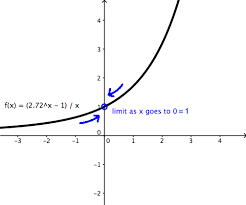
\includegraphics[scale=0.8]{../images.png}
\end{figure}

In the above graph, while the function is not defined at $0$, it approaches, or comes near to, $1$. 
There are several different "types" of limits and rules for calculating them. 

The first type of limit you could call an "easy" limit. 
All you have to do is plug in the number you are approaching for your variable, because the function doesn't violate any rules like we described above. 
So for example, if you have the limit

\begin{equation*}
    \lim\limits_{x\rightarrow 1} x
\end{equation*}

You would just get 1. 
The second type of limit could be called a "$\frac{0}{0}$" limit. 
It does violate the rules, and we have to do some algebraic manipulation to get it into a form we can work with. 
This might be done via factoring a polynomial, normalizing the denominator or numerator, or some such method.

A quick algebra side-note here on how to do these things. 
Factoring a polynomial mainly references factoring quadratics, or equations of the form $ax^2 + bx + c$ ($=0$). 
We factor the left side by using this general method: find the factors of $ac$ and see which add up to $b$. 
Note that you can change the signs of the factors, that is, if you have $ac = 10$ and the factors are $1, \, 2, \, 5, \, 10$, and $b = 3$, you can do $5-2 = 3$. 
After this, we then take those two numbers, $5$ and $-2$ and rewrite it as $ax^2 + 5x -2x + c$. 
We then put parentheses in: $(ax^2 + 5x) + (-2x + c)$. 
Finally, we factor out the biggest common number (or variable) out of each of the parentheses.

Let's do this with a real problem. 
\begin{equation*}
    x^2 - x - 12
\end{equation*}
For $ac$, we get $1\times -12$, or $-12$. 
For $b$, we get $-1$. 
The factors of $12$ are $1, \, 2, \, 3, \, 4, \, 6, \, 12$. $-4\times 3 = -12$ and $-4+3 = -1$. 
So now we write 
\begin{equation*}
    x^2 - 4x + 3x - 12
\end{equation*}
Now, we put in the parentheses and get
\begin{equation*}
    (x^2-4x)+(3x-12)
\end{equation*}
Now for the last step, factoring. 
For the first parenthesis, we can take out $x$, and in the second parenthesis, we can take out $3$, so we get
\begin{equation*}
    x(x-4)+3(x-4)
\end{equation*}
Note that if the two parenthesis' contents are not the same, then you have done something wrong. 
Now, we can rewrite this expression as 
\begin{equation*}
    (x+3)(x-4)
\end{equation*}
The equation is now factored.

The other thing of note here is rationalizing the denominator or numerator. 
Normally, we rationalize the denominator to get a radical out of the denominator, but we can also do this for the numerator. 
To do this, we multiply by expression on the numerator or the denominator over itself. 
Let's say we have the expression $\frac{\sqrt{x}}{1}$. 
Then we would multiply by $\frac{\sqrt{x}}{\sqrt{x}}$ and simplify. 
Note that if instead we had an expression like $\frac{\sqrt{x}+1}{1}$ we would multiply by $\frac{\sqrt{x}-1}{\sqrt{x}-1}$. 
We switched the sign on the $1$ from $+$ to $-$. This is called taking the "conjugate" of the expression.

With these tools in hand, we can now start solving the second type of limit. 
Let us take as an example 
\begin{equation*}
    \lim\limits_{x\rightarrow -3}\frac{x^2-x-12}{x+3}
\end{equation*}
We can clearly see that if we just plug it in, there will be a zero in the denominator. 
Instead, we can try employing an algebraic tool. 
You might recognize the quadratic on the top as the one we factored earlier. 
Let us then replace that expression with its factored form:
\begin{equation*}
    \lim\limits_{x\rightarrow -3}\frac{(x+3)(x-4)}{x+3}
\end{equation*}
Now, we can cancel the $x+3$ on the top and bottom of the fraction. 
This then leaves us with
\begin{equation*}
    \lim\limits_{x\rightarrow -3}x-4
\end{equation*}
The limit is now one of our "easy" limits, so we can simply plug in $-3$. The answer is $-7$.

Now we have our final type of limit, the "$\frac{\text{not zero}}{0}$" limit. 
This type of limit is a bit different from the other two types of limits. 
It requires a bit more intuition. As an example, let's say we are trying to solve the problem
\begin{equation*}
    \lim\limits_{x\rightarrow 0}\frac{1}{x}
\end{equation*}
To solve this, we must first solve
\begin{equation*}
    \lim\limits_{x\rightarrow 0^+}\frac{1}{x}
\end{equation*}
and
\begin{equation*}
    \lim\limits_{x\rightarrow 0^-}\frac{1}{x}
\end{equation*}
First, let's examine the second problem. 
The $+$ sign means it is a right limit - that is, we are approaching zero from the left. 
What does that mean? Well, let's say we have a number line like the one below.

\begin{figure}[H]
\caption{Approaching zero}
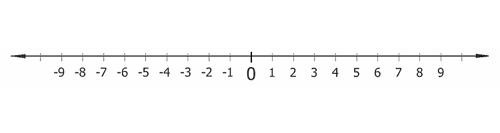
\includegraphics[scale=0.75]{../numberline.jpg}
\end{figure}

To approach from the right means that $x$ will be represented by tiny positive numbers, like $0.00001$ and $0.0000001$. 
They will get closer and closer to $0$. 
So, what does this mean? 
It means the answer to this particular limit will be whatever $\frac{1}{\text{really small positive number}}$ is. 
So let's take some examples. 
If we have $\frac{1}{0.00001}$ we get $100000$. 
If we have something closer to zero, like $\frac{1}{0.0000001}$ we get $10000000$. 
In other words, we are approaching infinity.
So the answer to this limit, approached from the right, is $+\infty$, or just $\infty$. 
Now, let's do the next one. 
This time, we are approaching zero from the left. Now we are dividing by small negative numbers. Try a few on a calculator and see what you get!

It turns out that this approaches $-\infty$. 
So the answer to the third limit in that list we started with is $-\infty$. 
Now, to solve the first limit. 
If we take the second two limits and their answer is the same, the first limit has a solution: the answer to the second two limits! 
However, the second two limits had different solutions. That means the answer to the first limit is undefined.

\section{Problems}
\begin{enumerate}
    \item $$\lim\limits_{x\rightarrow 3} 2x+5$$
    \item $$\lim\limits_{x\rightarrow 4} \frac{x^2-16}{x-4}$$
    \item $$\lim\limits_{x\rightarrow 9} \frac{\sqrt{x}-3}{x-9}$$
    \item $$\lim\limits_{x\rightarrow 0} \frac{1}{x^2}$$
    \item $$\lim\limits_{x\rightarrow 1} \frac{\sqrt{x}-1}{x-1}$$
\end{enumerate}

\section{Differential}

Differential calculus is all about finding the slope of a curve. 
First, let's consider a normal case, finding the slope of a straight line. 
We take in two points, and find the change in x and change in y ($\Delta x$ and $\Delta y$). 
This can be written as $\frac{\Delta y}{\Delta x}$ or $\frac{\text{rise}}{\text{run}}$.

\begin{figure}[H]
\caption{Average Slope}
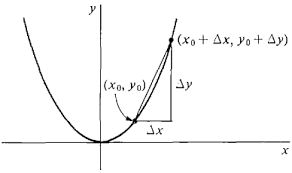
\includegraphics[scale=1]{download.png}
\end{figure}

The above diagram illustrates this process on a curve. 
We pick two points on the line and find the average slope. 
However, this process is clearly not very accurate. 
Imagine that we move the two points closer and closer together. 
The closer the points are, the more accurate the slope is for that section of the line, until both points are on top of each other, and we have a line that touches our curve at one point.
That is, we are finding instantaneous slope.
The derivative does that for the whole line, taking in a function and giving a new function that represents the slope. 
For example, let's say we shoot a cannonball.

\begin{figure}[H]
\caption{Trajectory of cannonball}
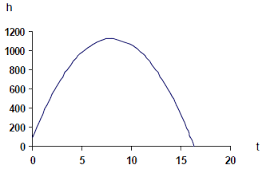
\includegraphics[scale=1]{imgres.png}
\end{figure}

Here, the y-axis represents the height of the cannonball in meters and the x-axis indicates time in seconds. 
Notice that at the beginning the slope is positive, until eventually the graph reaches its peak and the slope is zero, and then the graph starts going down and the slope becomes negative. 
The derivative of this graph would then look something like this:

\begin{figure}[H]
\caption{Derivative of trajectory of cannonball}
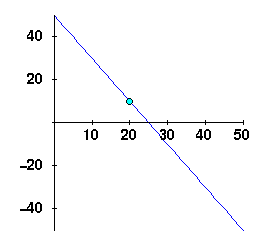
\includegraphics[scale=0.8]{derivative.png}
\end{figure}

This is what is happening "behind the scenes" when we calculate derivatives.
However, it is important to note that, going back to the example of the cannonball, where the cannonball started does not affect the slope. 
If the whole graph is shifted up or down, the slope stays the same (as long as the proportions are kept the same). 
This, it turns out, is why we need to add the $c$ in a indefinite integral. 

Derivatives and integrals are inverses of each other. 
That is, they undo each other, like division undoes multiplication and subtraction undoes addition. 
So, because when going from an integral back to a derivative there is some uncertainty which graph you are looking at (parallel lines, for instance, have the same slope, but they have different "heights"), you have to add the $c$ when solving an indefinite integral.

Below is a table with some solutions to various derivatives. Note that $c$ is a constant and $n$ is non-zero. Note that the $'$ symbol is pronounced prime, and is another way to write that we are taking the derivative. 


\begin{tabular}{c|c}
    $f(x)$ & $\frac{df}{dx} = f'$\\
    \hline
       $7$  & $0$ \\
        $c$ & $0$ \\
        $x$ & $1$ \\
        $cx$ & $c$ \\
        $x^2$ & $2x$ \\
        $cx^2$ & $2cx$ \\
        $x^3$ & $3x^2$ \\
        $x^n$ & $nx^{n-1}$ \\
        $\sin x$ & $\cos x$ \\
        $\cos x$ & $-\sin x$ \\
        $- \sin x$ & $- \cos x$ \\
        $-\cos x$ & $\sin x$
\end{tabular}

Like integrals, derivatives are distributive over addition.
There are some interesting rules that make working with derivatives easier: the product rule, the quotient rule, and the chain rule. 

Let's start with the chain rule. 
If we have a function within a function in a derivative, like $\sin(\cos(x))$, we can assign a name to each function, like $g(x) = \cos(x)$ and $h(x) = \sin(x)$, and then follow this simple rule: $h'(g(x)) \cdot g'(x)$. 
So what does this mean? 
Well, let's plug it in. 
Plugging this in gives $\sin'(\cos(x)) \cdot \cos'(x)$. 
So the derivative of $\sin$ is $\cos$, so we write $\cos(\cos(x))$ for the first part, and the derivative of $\cos$ is $-\sin$, so we write $-\sin(x)$ for the second part. 
So now we have $\cos(\cos(x)) \cdot -\sin(x)$. 
This is the derivative of our original function.

Now, let's examine the product rule. 
If we have two functions, $u(x)$ and $v(x)$, and we want to take the derivative of $u\cdot v$, then we can do $u \cdot \frac{dv}{dx}+ v\cdot\frac{du}{dx}$. 
In other words, we multiply the first function by the derivative of the second function and then add the second function times the derivative of the first. 
For example, if we have $\sin(x)\cdot\cos(x)$ we would do $u(x) = \sin(x)$ and $v(x) = \cos(x)$. 
Then we would plug it in to our formula: $\sin(x)\cdot\frac{d}{dx}\cos(x) + \cos(x)\cdot\frac{d}{dx}\sin(x)$ which simplifies to $\sin\cdot -\sin(x) + \cos(x)\cdot\cos(x)$ or $-\sin^2(x)+\cos^2(x)$, which is our derivative of the original function.

Finally, the quotient rule. 
If we have two functions, $g(x)$ and $h(x)$, and we wish to take the derivative of $\frac{g(x)}{h(x)}$, we can follow the rule $\frac{g'(x)h(x)-h'(x)g(x)}{[h(x)]^2}$. 
While this may look rather complicated, it really isn't too bad. 
Let's use the example of $g(x) = \sin(x)$ and $h(x) = \cos(x)$. 
We plug it all in to get $\frac{\sin'(x)\cdot\cos(x) -\cos'(x)\cdot\sin(x)}{\cos^2(x)}$
which simplifies to $\frac{\cos(x)\cdot\cos(x)--\sin(x)\cdot\sin(x)}{\cos^2(x)} = \frac{\cos^2(x)+sin^2(x)}{\cos^2(x)} = \frac{1}{\cos(x)}$ (this top part simplifes due to the Pythagorean Identity). 
So therefore, $\frac{1}{\cos(x)}$ is our derivative.

\section{Problems}
\begin{enumerate}
    \item $5x$
    \item $6x^3 - 9x + 4$
    \item $2t^4 - 13t$
    \item $x^{-1}$
    \item $\sqrt{x}$
\end{enumerate}

\section{Integral}

The point of the integral is to find the area under a curve. 
One of the interesting applications of integration is finding the displacement of an object - the displacement corresponds to an object's trajectory; that is, the area under a graph of velocity versus time is displacement.

While we don't actually need to do the following, this is generally what is happening. 

\begin{centering}
\begin{figure}[H]
\caption{Riemann Sum}
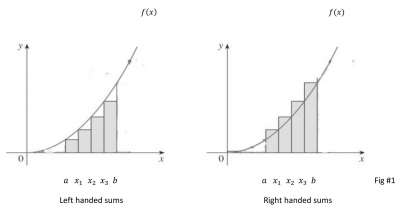
\includegraphics[scale=0.8]{rieman.jpg}
\end{figure}
\end{centering}

Basically, we pick a specified width, let's say $w$. 
Then, we create several rectangles, with a width $w$ and a height that is just under the curve we are trying to find the area of. 
Then, we do this again, but this time the height is just above the curve. 
We take the average of the two numbers, and get the area of the curve. 
The smaller we make $w$, the more accurate the number, and at width $0$, we basically have lines, which fit the curve perfectly. 
This is the point of an integral.

Below is a table of some of the basic outputs of integrals. Some of these will make more sense after going through derivatives.

\begin{tabular}{l|l}
    $f(x)$ & $\int f(x) \, dx$\\
    \hline
     $0$ & $0+c$ \\
     $1$ & $x+c$ \\
     $D$ & $Dx+c$ \\
     $2x$ & $x^2 + c$ \\
     $x$ & $x^2/2 + c$ \\
     $x^2$ & $x^3/3 + c$ \\
     $x^n$ & $x^{n+1}/n+1 + c$
\end{tabular}

In these, $c$ and $D$ are constants and $x$ is some variable.

Note that after every integral, we must put $dx$ or $dt$ or $d$ and then whatever variable we are using in our integral. 
The second important thing to note is that these results have $c$ after them because they are ``indefinite'' integrals - that is, because we don't have a specific bound on the integral, we must add a constant $c$ to show that there is some range in what the answers will be. 
This is again something that will make more sense after going over derivatives.

So there are indefinite integrals, but there are also "definite" integrals. 
We write them as $\int^b_a$. Basically, let's say we have the integral $\int x \, dx$. 
We integrate the inside according to the table, getting $x^2/2$, but instead of adding the constant $c$, we then plug in $b$ and $a$ in for $x$ as follows: 
\begin{equation*}
    (b^2/2) - (a^2/2)
\end{equation*}

This gives our answer, and we do not need to put in $c$.

There is another important thing about integrals. For an integral such as $\int x+x \, dx$, we can change this into

\begin{equation*}
    \int x \, dx + \int x \, dx
\end{equation*}

We can also factor out constants; for example, given $\int 2x + 3x \, dx$, we can change this into 

\begin{equation*}
    2\cdot \int x \, dx + 3 \cdot \int x \, dx
\end{equation*}

Also remember that you can simplify within a problem; i.e., given $x(x^2 + x^3)$ you can then multiply and get $x^3 + x^4$. 
Finally, there is a helpful rule for integrals - the product rule. 
If you have a function $v(x)$ and a function $u(x)$, and you wish to find the derivative of $u(x)\cdot v(x)$, you can follow the rule $u\cdot v - \int v\frac{du}{dx}\, dx$. 

\section{Problems}
Solve the following integrals:

\begin{enumerate}
    \item $\int x \, dx$
    \item $\int x^2-5 \, dx$
    \item $\int^5_0 x^2 \, dx$
    \item $\int^5_3 x^2 \, dx$
    \item $\int^5_3 x^2 + 1 \, dx$
\end{enumerate}

\section{Applications}
Now we get to the most interesting part of calculus: its applications. 
Here, we are going to focus on only a few applications, but there are many applications of calculus, across many fields, such as economics, sociology, physics, mathematics itself, chemistry, astronomy, and others. 
Calculus is key in many fields.

The main application we are going to look at is work, as defined by physics. 
Interestingly, there is an integral definition of work - that is, work can be defined using an integral.

\begin{equation*}
    \int^b_a f(x) \, dx
\end{equation*}

What does this mean? 
Well, first, $f(x)$ is a function representing force, where $x$ is displacement, which, as Newton's second law states, is $F = ma$ - that is, force is mass times acceleration. 
Second, $b - a$ should equal the displacement, or how much the object is moved. This is because $b$ and $a$ are what we are substituting for $x$, which is displacement.
This is easier to illustrate with a few problems.

For example, let's say we have a bowling ball, rolled with a force equal to the function $f(x) = 2x+3$ (where the resulting number is in Newtons). 
We want to find out how much work it takes to roll it from the start of our lane down to the end of the lane, 10 meters away.

Well, here, this is easy. All we do is plug in the numbers into our formula for work! 

\begin{equation*}
    \int^{10}_0 2x+3 \, dx
\end{equation*}

Remember that $a$ and $b$ together represent displacement. 
We're rolling the bowling ball from the start, $0$, to the end of the lane, $10$ meters away. 
So that represents $a$ and $b$ respectively. 
The force, $f(x)$, is simple to plug in. 
So now, we follow the rules for integrating. 
In this case, we get $2\frac{x^2}{2}+3x\mid^{10}_0$. 
Note that this last part, the line with the superscripts, is just a bit of notation, saying that we plug in $10$ and $0$ and subtract according to the rules of definite integrals. 
It just allows us to integrate and write that down. 

So now that we have this, we plug it in as we would for normal definite integrals, and so we get $(2\cdot\frac{10^2}{2}+3\cdot 10) - (2\cdot\frac{0^2}{2}+3\cdot 0)$ and then we simplify. 
The whole second half comes to zero, so we now have $2\cdot\frac{10^2}{2}+3\cdot 10$. 
Then, we have $2\cdot \frac{100}{2}+ 30$ or $2\cdot 50 + 30$ or $130$. 
Now we look at units. 
We have meters and newtons, so now when we multiply those two, we have joules (a unit of work). 
So our answer is $130$ joules. 
Note that it is very important to keep track of your units. If you don't know a unit of force, work, or distance, look it up! Think logically.

A quick note on Hooke's Law: when considering the work required to stretch a spring, you can assume that the force ($f(x)$) needed to stretch a spring a distance $x$ beyond its natural length is proportional to $x$. 
In other words, we have $f(x) = cx$ where $x$ is the distance the spring is stretched and $c$ is some constant.

\section{Problems}
For the second problem, the spring can be assumed to obey Hooke's Law.

\begin{enumerate}
    \item If throwing a baseball requires a force equivalent to $f(x) = 5x^2$ pounds then find the work necessary to throw a baseball from third to first base (about $127$ feet).
    \item If a ten-pound force stretches an elastic spring one inch, how much work is done in stretching the spring one foot?
\end{enumerate}

\section{Multivariable Calculus}
Here we will examine only one part of multivariable calculus, partial derivatives.
Partial derivatives are actually not too difficult once you know how to do normal derivatives.
The basic principle is this: given a function, take the derivative of it with respect to one variable, while treating the other variables as constants.
How does this work? Well, let's take as an example the function $f(x,y)=3x-2y^4$.
We would first take the derivative of this function with respect to $x$, treating $y$ as a constant. 
So, the derivative of $f_x$ would equal $3$ - the second term vanishes because $y$ is a constant. 
Then, we would take the derivative of the function with respect to $y$, treating $x$ as a constant.
The derivative of $f_y$ would equal, therefore, $-8y^3$. 
So the partial derivative of $f(x,y)$ is $f_x=3, f_y=-8y^3$.
Let's do this again with a more complicated function. Given $f(x,y,z)=xy^2z^3+3yz$, we would get $f_x=y^2z^3$, $f_y=xz^32y+3z$, and $f_z=xy^23z^2+3y$.
The other important thing to mention is how partial derivatives are written. Instead of writing $\frac{d}{dx}$ or $\frac{dx}{dy}$ to represent derivatives (the second representing the derivative of the function $x$ with respect to $y$ and the first representing the derivative of what follows with respect to $x$) we write $\frac{\partial}{\partial x}$ or $\frac{\partial x}{\partial y}$ - the $\partial$ symbol represents the derivative.
\section{What Next?}
What is explained here is just a taste of calculus, and isn't completely formalized (for example, derivatives and integrals are actually defined using limits). There are other fields of calculus that will be useful to you should you choose to study these subjects further. A more rigorous study of single-variable calculus will be necessary for  these. Multivariable calculus as a whole is also recommended; here we only covered partial derivatives. Vector calculus will also be useful, expanding the topics of linear algebra (see chapter two) to calculus. Finally, it is suggested that you study ordinary and partial differential equations. 
\chapter{Linear Algebra}
\section{Vectors}
Imagine an arrow, floating in space. Try to describe where in space it is to someone else. It's difficult, isn't it?
Now, imagine that same arrow on the Cartesian plane, with its tail on the origin. Describe where the arrow is by giving the coordinates of the tip of the arrow, in the form $\begin{bmatrix}x\\y\end{bmatrix}$.
Much easier, right? Well, we call these arrows vectors, and they represent both magnitude (the length of the vector) and direction (which way the vector is pointing). 
\begin{center}
\begin{figure}[H]
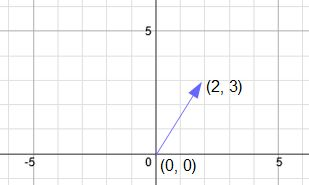
\includegraphics[scale=0.7]{visualvectordotproduct1.jpg}
\end{figure}
\end{center}
In the figure above, you'll see how we look at vectors. The vector is represented by the coordinates of the tip of the vector, with the tail on the origin. We can perform operations on vectors, like adding. A diagram of this is shown below.
\begin{figure}[H]
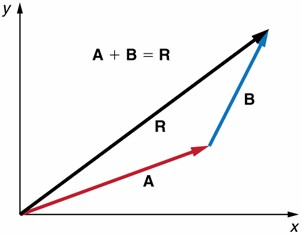
\includegraphics[scale=0.5]{Figure_03_03_05a.jpg}
\end{figure}
Geometrically, adding is done by placing the second vector's tail at the tip of the first vector, and drawing the new vector from the tail of the first to the tip of the second. Mathematically, this is done by doing $\begin{bmatrix}x_1\\y_1\end{bmatrix}+\begin{bmatrix}x_2\\y_2\end{bmatrix}=\begin{bmatrix}x_1+x_2\\y_1+y_2\end{bmatrix}$. So adding vectors is fairly simple, and subtraction of vectors operates on the same principle.
We can also multiply vectors by normal numbers, or scalars.
\begin{center}
\begin{figure}[H]
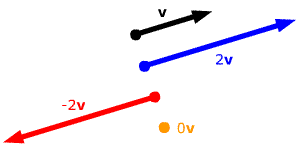
\includegraphics[scale=0.5]{mult2.png}
\end{figure}
\end{center}
The scalar stretches the vector if it is positive and greater than one, keeps the vector the same if it is one, shrinks the vector while less than one and greater than zero, makes the vector into a point if it is zero, and flips the vector and stretches or shrinks it as described if it is negative.
In this, it is just like multiplication of two normal numbers. The next important thing about vectors is that there are basis vectors. Imagine a small vector, taking up one unit of each of the axes on the coordinate plane. 
\begin{center}
\begin{figure}[H]
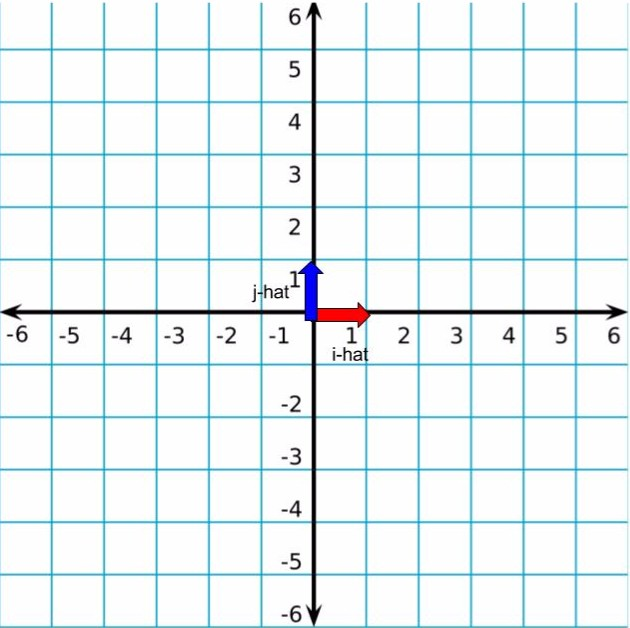
\includegraphics[scale=0.25]{basis.jpg}
\end{figure}
\end{center}
These two vectors are called $\hat{i}$ (read i-hat) and $\hat{j}$ (read j-hat). What's interesting is that all vectors are composed of these basis vectors (a new basis vector is added for each dimension). How? Well, let's say we have a vector $\mathbf{v}$ (variables for vectors are commonly bolded or written with an arrow on top). We can write it as a scalar $a$ multiplied by the basis vector $\hat{i}$ plus another scalar $b$ multiplied by the basis vector $\hat{j}$. You can also pick different basis vectors, by changing the axes, and get a new logical system.
\section{Matrices}
So we have this concept of vectors. But linear algebra isn't just about vectors, it also talks about matrices. Basically, matrices represent transformations of the coordinate plane, and all the vectors in it. A transformation is a function, with vector inputs and outputs. The functions, however, must be linear. This can be thought of geometrically as keeping all of the gridlines of the coordinate plane straight and parallel, and keeping them from getting curved. The other rule is that the origin must remain fixed in place.
So, how do matrices represent this transformation? Well, they just show where $\hat{i}$ and $\hat{j}$ end up. So, if $\hat{i}$'s coordinates are $\begin{bmatrix}\hat{i}_x\\\hat{i}_y\end{bmatrix}$ and $\hat{j}$'s coordinates are $\begin{bmatrix}\hat{j}_x\\\hat{j}_y\end{bmatrix}$, the matrix representing that transformation would be $\begin{bmatrix}\hat{i}_x & \hat{j}_x\\\hat{i}_y & \hat{j}_y\end{bmatrix}$. We can multiply this matrix by any vector to get what the coordinates of that vector would be in the new system.
Suppose, however, that we wish to do two transformations. Instead of applying each matrix separately, we can multiply the two matrices and apply that new matrix to the vector. Suppose we have two matrices, how do we multiply them? We can do
\begin{equation*}
\begin{bmatrix}a&b\\c&d\end{bmatrix}\begin{bmatrix}e&f\\g&h\end{bmatrix}=\begin{bmatrix}ae+bg&af+bh\\ce+dg&cf+dh\end{bmatrix}
\end{equation*}
\section{Determinants}
The next important thing about linear algebra is the determinant. Basically, the deteriminant is the area of one grid square.
\begin{center}
\begin{figure}[H]
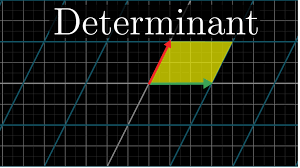
\includegraphics[scale=0.5]{determinant.png}
\end{figure}
\end{center}
The determinant changes depending on the basis vectors. Because a matrix represents a linear transformation, and therefore the basis vectors, we can calculate the determinant of a 2x2 matrix as follows:
\begin{equation*}
\det\left(\begin{bmatrix}a&b\\c&d\end{bmatrix}\right)=ad-bc
\end{equation*}
Calculating the determinant is different if you have a 3x3 matrix (remember that the size of a matrix represents the number of dimensions the transformation is taking place in).
\section{Dot Product}
A dot product is a simple function that takes in two vectors and outputs a scalar as follows:
\begin{equation*}
\begin{bmatrix}a\\b\end{bmatrix}\begin{bmatrix}c\\d\end{bmatrix}=ac+bd
\end{equation*}
It will be useful later on in these notes.
\section{Solving Systems of Equations}
One of the many useful applications of linear algebra is solving systems of equations. For example, let's say we have the system of equations $2x+2y=-4$ and $x+3y=-1$. We can solve this by putting all the coefficients in a matrix, all the variables in a vector, and all the constants in a vector:
\begin{equation*}
\begin{bmatrix}2&2\\1&3\end{bmatrix}\begin{bmatrix}x\\y\end{bmatrix}=\begin{bmatrix}-4\\-1\end{bmatrix}
\end{equation*}
We can solve this by multiplying each side by the inverse of the matrix. This makes sense - if we are solving a simpler equation, say $5x=10$, we solve by dividing each side by $5$, because division is the inverse of multiplication. The inverse of the matrix is a matrix that, when multipled by the original matrix, produces the identity matrix. The identity matrix is kind of like $1$ - when applied to other matrices, it doesn't change anything. The identity matrix is $\begin{bmatrix}1&0\\0&1\end{bmatrix}$. You can test it for yourself. To find the inverse of a 2x2 matrix, we can follow the following rule (where $A$ is the original matrix, and $A = \begin{bmatrix}a&b\\c&d\end{bmatrix}$):
\begin{equation*}
\frac{1}{\det(A)}\begin{bmatrix}d&-b\\-c&a\end{bmatrix}
\end{equation*}
The rule is different, and more complicated, for 3x3 matrices. In the case of our system of equations from earlier, the inverse is $\begin{bmatrix}\frac{3}{4}&-\frac{1}{2}\\-\frac{1}{4}&\frac{1}{2}\end{bmatrix}$. Multiplying it by both sides produces the equation
\begin{equation*}
\begin{bmatrix}x\\y\end{bmatrix}=\begin{bmatrix}-\frac{11}{4}\\-\frac{5}{2}\end{bmatrix}
\end{equation*}
And so we have the solutions to our system.
\section{What Next?}
This overview of linear algebra really only scratches the surface, and it covers most of it in only two dimensions. There are other interesting functions (the cross product, for instance), subfields (such as multilinear algebra, which is actually rather relevant to general relativity), such things as vector spaces, and other interesting areas of study. It is recommended that the reader make an attempt to examine some of these areas.
\section{Problems}
\begin{enumerate}
\item Add the vectors $\begin{bmatrix}3\\2\end{bmatrix}$ and $\begin{bmatrix}5\\1\end{bmatrix}$.
\item Multiply the matrices $\begin{bmatrix}3&2\\6&1\end{bmatrix}$ and $\begin{bmatrix}5&3\\4&6\end{bmatrix}$.
\item Find the dot product of the vectors from problem one.
\end{enumerate}
\part{General Relativity}
\chapter{Introduction}
General relativity is a generalization of special relativity to include gravity. It has lead to many important discoveries,
as well as the whole field of cosmology. It is also one of the two main advancements of the 20th century, the second being, of course,
quantum mechanics. It is therefore important to understand at least the very basics of general relativity.
Note that this description is not completely rigorous, and tries to get the point across intuitively as well as mathematically.
Also worth pointing out is that you will need to understand the math explained in part one, especially the calculus. It will be very
hard to understand the rough derivation if you do not.
\section{Principle of Equivalence}
One of the first big things Einstein did was look at the following situation. Imagine you are in a box with no windows, on Earth, being pulled down
by gravity (or a force $g$). Now, imagine you are in a rocket, also with no windows, in outer space, accelerating with that same force $g$. 
\begin{figure}[H]
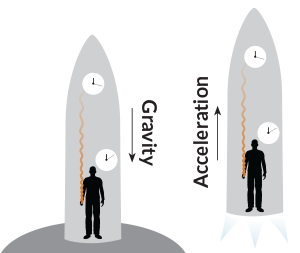
\includegraphics[scale=0.5]{equiv.png}
\end{figure}
Einstein said that there is no experiment that you could do to distinguish these situations. Try to come up with an experiment that you
think would distinguish the two. Why might it be wrong? I guarantee, however, that it is incorrect. 
So, these two situations are sort of the same - there's a fundamental equivalence between the two.
Now, let's imagine we are in that rocket again.
\begin{figure}[H]
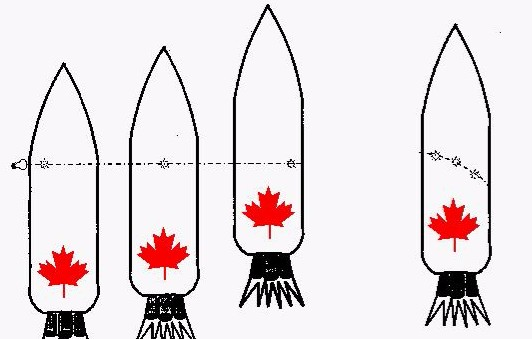
\includegraphics[scale=0.5]{relgen3.jpg}
\end{figure}
Imagine shining a flashlight from one side of the rocket to the other. From the point of view of an observer on the Earth,
the light goes in a straight line, but since the rocket is accelerating, the light appears to bend down from the point of view of
the observer in the rocket. Because the light is bending here, and we established that there is a fundamental equivalence between
this situation and that box on the Earth, the same thing must happen there, and it does. But we can draw a more general conclusion
from this: namely, that light bends in a gravitational field. This explained something interesting that had happened. In a solar
eclipse earlier, astronomers had seen a star that should have been behind the sun. What had happened is shown in the following diagram:
\begin{figure}[H]
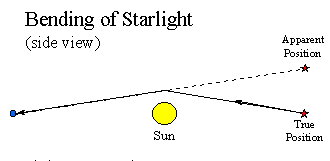
\includegraphics[scale=0.75]{bend.png}
\end{figure}
The star's light was bent by the sun's gravitational field. If instead of accounting for the bend, you looked straight along the line
of light, the star appeared to be in a different position.
\section{Curved Spacetime}
There is another interesting implication of the idea that light is bent by a gravitational field. To understand it, we have to look
at Newton's law of gravity. He said that the gravitational force between two objects is $F=\frac{Gm_1m_2}{r^2}$, where $m_1$ is 
the mass of the first object, $m_2$ is the mass of the second object, $r$ is the distance between the two masses, and $G$ is a constant.
Now, let's say we are looking at how light is curved by the sun. The mass of the sun is a whopping $1.989 \times 10^30$ kilograms. 
Light is made up of photons, which have a mass of...zero kilograms. Can you see the problem here? The whole equation will come out to
zero, yet we know that the gravitational force is not zero in this case! Newton's law, which was established for hundreds of years, is
wrong. 

So what is the right approach? Well, Einstein said that gravity isn't actually a force, but the result of curved "spacetime". You can 
imagine the three dimensions of space plus a fourth of time being a flat rubber sheet. When a mass, like a bowling ball is placed
on the sheet, the sheet bends. A lighter mass, such as a tennis ball, when placed on the sheet near the bowling ball will roll toward
the bowling ball - kind of like gravity. However, in this case we only have two-dimensional space being warped. A better image
would be something like the image below:
\begin{figure}[H]
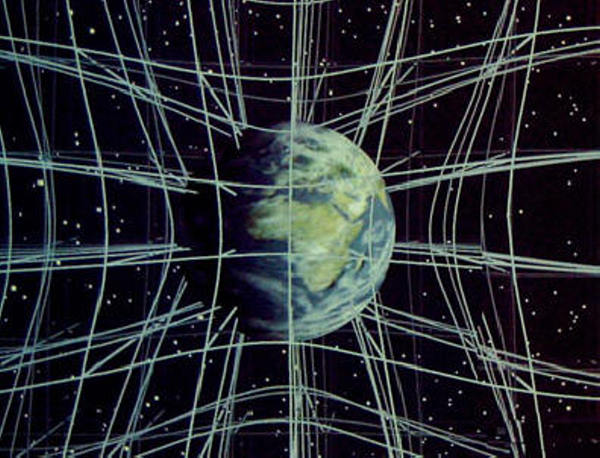
\includegraphics[scale=0.25]{warpspace.jpg}
\end{figure}
However, this still isn't a perfect image, because time isn't warped in this picture, but it's a good enough mental image for now.
So, to summarize, Newton said that gravity was caused by the attraction of two objects, but Einstein said that gravity wasn't
really a thing - objects were just taking the shortest possible path in curved spacetime. 

There is another interesting thing to look at in curved spacetime - spacetime graphs. The first thing to note is the normal three
dimensions of space graphed:
\begin{figure}[H]
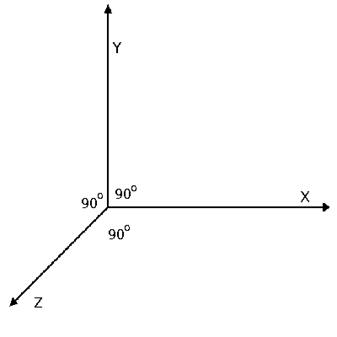
\includegraphics[scale=0.5]{3d.jpg}
\end{figure}
Note that the three axes are at right angles to each other (in math speak, they are orthogonal). If we were to add an axis for the
dimension of time, it would have to be at right angles to all the other axes. Needless to say, this is rather hard to visualize,
so to keep it simple, we're going to stick to one dimension of space and one of time in our graphs. So imagine we have an object 
that is stationary - perhaps your desk, or maybe a book on your shelf. It would be graphed as a straight line up. Why is this? 
Well, the object may not be moving, but time is passing! So there is a straight
line to represent a lack of movement through space, but a steady movement through time. Now, imagine that an object is moving at
a constant velocity. That would look something like this:
\begin{figure}[H]
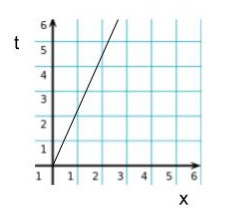
\includegraphics[scale=0.5]{constantv.jpg}
\end{figure}
It is moving through both space and time, so it is a diagonal line. Another spacetime diagram that is of interest - what would an object
look like that is accelerating?
\begin{figure}[H]
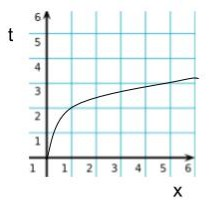
\includegraphics[scale=0.5]{acceler.jpg}
\end{figure}
The line is curved - it is reaching the same location in less time. Finally, it is important to note that the object cannot move
faster than the speed of light. It is common practice to draw the speed of light as 45 degrees from the x-axis, so anything at an
angle less than 45 degrees to the x-axis is expressly forbidden, as demonstrated by the following diagram.
\begin{figure}[H]
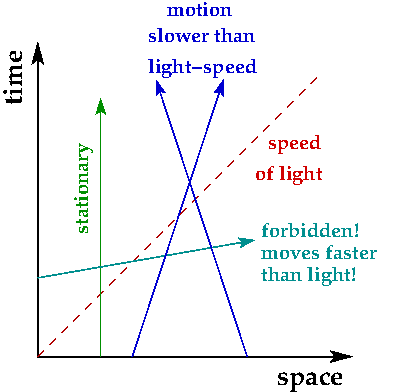
\includegraphics[scale=0.5]{light.png}
\end{figure}
These are some of the very basic ideas of general relativity. In the next chapter, we will look at Einstein's field equations, which describe the exact relationships between curvature, mass, and energy.
\chapter{Einstein's Field Equations}
\section{Summary}
And so, after quite a bit of text, we come to the meat of the matter: the Einstein field equations. Without further ado, here they are:
\begin{equation*}
R_{\mu\nu}-\frac{1}{2}g_{\mu\nu}R+g_{\mu\nu}\Lambda=\frac{8\pi G}{c^4}T_{\mu\nu}
\end{equation*}
While this may look deceptively simple, they are actually quite complicated. Here, $\mu$ and $\nu$ represent the dimensions of spacetime.
You may wonder how this is equations, plural. It may only look like one equation, but in fact, $\mu$ and $\nu$ are able to take 
four different values, representing the four different dimensions of spacetime. They show up at four different spots, resulting in 
sixteen variations of the same equation. However, six turn out to be duplicates, so there are ten Einstein field equations.

What are all the various letters and variables here? Well, we've already established what $\mu$ and $\nu$ are. $G$ we've already seen;
it is Newton's graviational constant. The speed of light is $c$, which is something you may already be familiar with, along with $\pi$
and the other constants on the right hand side. $R_{\mu\nu}$ is called the Ricci curvature tensor. $g_{\mu\nu}$ is the metric tensor.
(We will get into later what these different things mean.) $R$ is the curvature scalar. $T_{\mu\nu}$ is the stress energy momentum tensor.
Finally, $\Lambda$ is the cosmological constant.

This equation balances two things. On the left, the various terms represent the curvature of spacetime. On the right, the various terms
represent mass and energy. In other words, the equations basically say this: mass tells spacetime to curve, and spacetime tells mass
how to move.

\section{Rough Derivation}
\chapter{Solutions to the Field Equations}
\section{Schwarzschild Solution}
actual derivation
\section{Big Bang}
summary
\section{Gravitational Waves}
summary


\nocite{bluebrown}
\nocite{khanacademy}
\nocite{passcalculus}
\nocite{mitocw}
\nocite{paulmath}
\nocite{apostoli}
\nocite{apostolii}
\nocite{spivak}
\nocite{cartoon}

\bibliographystyle{plain}
\bibliography{resources}
\addcontentsline{toc}{section}{References}
\begin{appendices}
\chapter{Circles with Calculus}
Here is the text of a conversation between a teacher and a student, discussing an interesting problem:\\
Teacher: Do you know the area of a circle with radius $r$?\\
Student: $\pi r^2$, and circumference is $2\pi r$. \\
Teacher: Yeah, okay. Prove it. With calculus. Any idea how to do that?\\
Student: Let me see...it involves an integral, I'm guessing. And then, maybe a definite one, over the interval $0$ to $\pi$? No, that's not right. Well, maybe. but what are you integrating over? Not $r$, if it is a definite integral. Let me think about this more intuitively.
You rotate the radius around $\pi r$ times, I suppose, to get the area (does that make sense?) and then it might be instead over the interval $\int^{\pi}_r$,\\
Teacher: Let's think of the disk as a set of concentric rings.\\
Student: Okay, then, hmm, inside, you'd have some variable $x$, and how would that look...maybe $x^2$? Or something?
So then integrating that you get $x^3/3$ - 
no wait, that doesn't make sense either, because then you are subtracting.
Okay, different way.
$2\pi r$ is the circumference of the circle,
so then we can say $2\pi r$ over the interval $0$ to $r$,  I think.
So then you'd have the integral $\int^r_0 2\pi r \, dr$,
and then you'd get $\frac{2\pi r^2}{2}\mid^r_0$.\\
Teacher: Okay, what does that become?\\
Student: Well, $\frac{2\pi r^2}{2}-\frac{2\pi 0^2}{2}$, and
the second part all becomes zero, so now you have $\frac{2\pi r^2}{2}$...
and then $\pi r^2$!\\
Teacher: Now review in your mind how you got that answer. You imagine a bunch of rings, each of radius $r$ and length $2 \pi r$.
If you give that ring a little bit of radial extent $dr$, the area of that new thing is $2 \pi r \times dr$.\\
Student: Radial extent is how thick the ring is, right?\\
Teacher: Yes. Then you summed (i.e. integrated) from 0 to $R$ and got $\pi R^2$.\\
Student: I wonder how you prove $2\pi r = \text{circumference}$.\\
Teacher: Do you know how to relate arc length to angle?
I.e., what a radian is?\\
Student: Barely...\\
Teacher 2: Well, that's the point where it gets tricky - one often defines $2\pi$ as the ratio of a circle to its radius, so there's nothing to prove.
There are other definitions (involving more math) of $\pi$ in which $C = 2\pi r$ is an actual theorem but I have to admit that I don't actually know how to derive it from them.\\
Teacher: I was hoping to prove that the circumference of a circle is equal to the radius times a constant.\\
Teacher 2: Ah, nevermind then. Carry on.\\
Teacher: Suppose I move a little bit horizontally $dx$ and a little bit vertically $dy$.
How far did I move in total?\\
Student: Well, maybe $\sqrt{dx + dy}$? I don't know if that's what you are looking for.\\
Teacher 2: Actually, the inside would be squared - $ds=\sqrt{dx^2+dy^2}$.\\
Teacher: Okay, so the equation for the points on a circle is $$x = R \cos(\theta) \qquad y = R \sin(\theta)$$.
 Can you write $dx$ in terms of $d\theta$?\\
Student:  I think you'd say $d(R \cos(\theta)$ - right?\\
Teacher: Yeah, so assume $R$ is constant...\\
Student: Then would you get $-\sin(\theta)$?\\
Teacher: Close. What is $dx / d\theta$? Have you done derivatives of$\sin$ and $\cos$?
Student: Well, derivative of $\sin$ is $\cos$, derivative of $\cos$ is $-\sin$, derivative of $-\sin$ is $-\cos$, and the derivative of $-\cos$ is $\sin$ (I think).\\
Teacher: Right, yeah. \\
Student: I'm kind of confused on what I'm doing with $dx/d\theta$, I guess.\\
Teacher: Well, $x = R \cos(\theta)$, so $dx/d\theta = \cdots$. You already said it.\\
Student: $-\sin(\theta)$?\\
Teacher: Yeah, so what's $dx$?\\
Student: The same thing?\\
Teacher: Nope, $dx = - R \sin(\theta) d\theta$.
We're not being careful about what $dx$ means by itself here, but let's just go with it.
The meaning is intuitively clear, I think.
Okay, so what's $dy$?\\
Student: $-R\cos(\theta)$?\\
Teacher: Where'd the minus come from, and where's the $d\theta$?\\
Student: I don't really know.\\
Teacher: $dy = R \cos(\theta) d\theta$
Does that make sense?
$y = R \sin(\theta) \rightarrow dy/d\theta = R \cos(\theta) \rightarrow dy = R \cos(\theta) d\theta$\\
Student: Hmm, I think so.
It makes sense, but I'm not sure, given another problem, that I could do it.\\
Teacher: Which bit is confusing?\\
Student: What exactly the $dy/d\theta$ means, exactly, I suppose - which equation are we finding the derivative of?\\
Teacher: We have two equations: $$x = R \cos(\theta) \qquad y = R \sin(\theta)$$
Those give you the x and y coordinates of the points on a circle, as you vary the angle $\theta$.
$dx/d\theta$ tells you how $x$ changes as we change the angle $\theta$.\\
Student: And then $dy/d\theta$ - how $y$ changes as we change $\theta$?\\
Teacher: Yeah. As you change the angle going around the circle, both x and y change!\\
Student: But wouldn't $R$, being a constant, vanish from the derivative?\\
Teacher: Nope. If I have $y = a x$ then $dy/dx = a$.\\
Student: Oh, that makes sense, sorry.\\
Teacher: No problem. So we have $$dx = - R \sin(\theta) d\theta \qquad dy = R \cos(\theta) d\theta$$\\
Student: Okay, I think I follow now.\\
Teacher: Cool. We also know, as you said, that if we move a bit in x and y, the total distance traveled is $$ds = \sqrt{dx^2 + dy^2}$$\\
Student: Right. \\
Teacher: So! Plug it in and see what you get. \\
Student: $ds = \sqrt{(-R\sin(\theta)d\theta)^2+(R\cos(\theta)d\theta)^2}$ - convoluted madness.
Simplifying gets
$\sqrt{(-R\sin (x)dx)(-R\sin(x)dx)+(R\cos(x)dx)(R\cos(x)dx)}$.\\
Teacher: Alright, but you can simplify that a lot. Multiply stuff together...\\
Student: Um, let's see, $R^2 \sin^2(x)dx$ for the first part?\\
And then plus $R^2\cos^2(x)dx$, right?\\
Teacher: Actually wait a second... $dx = -R \sin(\theta) d\theta$
You're plugging $dx$ and $dy$ into the $ds$ formula...\\
Student: Let me try this again.\\
Teacher: What's $dx^2 = (-R \sin(\theta) d\theta)^2$? $= R^2 \sin(\theta)^2 d\theta^2$.
So do the same for $dy^2$.\\
Student: So it'd be $\sqrt{R^2\sin(\theta)^2+R^2\cos(\theta)^2d\theta^2}$?\\
Teacher: YES!
Now factor out the stuff you can factor out...
Oh, and you forgot the $d\theta^2$ in the first term.\\
Student: Let's see, $R^2$, and $d\theta^2$,
so then we're left with $Rd\theta\sqrt{\sin(\theta)^2+\cos(\theta)^2}$?\\
Teacher: No. Forgot to square-root the stuff you pulled from the square root.
What's $\sin^2 + \cos^2$?\\
Student: Oh duh, one, the Pythagorean identity,
so $Rd\theta$,
because $\sqrt{1} = 1$
and one times anything = anything.\\
Teacher: Yes.
So you have $ds = R d\theta$.
This is a very nice result: the length of an arc of a circle is equal to the radius times the angle of that arc.
This is, actually, how angle is usually defined, but here we derived it from the starting point that a circle is defined by $x = R \cos(\theta)$ and $y = R \sin(\theta)$.
Now, how much arc length do you get if the angle goes from 0 to $2\pi$?\\
Student: Not sure...$2\pi$?\\
Teacher: Well, let's just do it. $$s_\text{total} = \int_{\theta=0}^{2\pi} R d\theta$$
$$=R \int_{\theta=0}^{2\pi} d \theta = ?$$\\
Student: $2\pi R$ - 
the circumference of the circle!
Which makes sense because $2\pi$ is a full revolution around!\\
Teacher: Right! You actually just did some multivariable calculus.
Remember we started with the Pythagorean thingy $ds = \sqrt{dx^2 + dy^2}$.
That tells you the length of a bit of curve in the 2D plane.
Then you used a parametrization of the circle, i.e. $x = R \cos(\theta)$ and $y = R \sin(\theta)$ to figure out $dx$ and $dy$ in terms of a single variable $\theta$, and then you did the integral to get the total path length.\\
Student: oh...wow, that's cool!\\
Teacher: Yes, it is!
 \\
A more rigorous proof of this is left to the reader if they are interested.
\chapter{Worked Solutions}
A few of the problems have been taken from Apostol's Calculus, Volume 1.

Integrals: 
\begin{enumerate}
\item $\int x \, dx = \frac{x^2}{2}+c$ For this one, all you have to do is use the table given. 
Because it is an indefinite integral, don't forget to add $c$!
\item $\int x^2 - 5 \,dx = \int x^2 \, dx - \int 5 \, dx = \frac{x^3}{3}-5x + c$ Remember that the integral is distributive over addition and subtraction. 
Also, remember that there is only one $c$ added to the solution of any indefinite integral.
\item $\int^5_0 x^2 \, dx = \frac{x^3}{3}\mid^5_0 = \frac{5^3}{3}-\frac{0^3}{3}=\frac{5^3}{3}=\frac{125}{3}$ Remember that $\mid^5_0$ is simply a piece of notation that allows us to keep track of what we are integrating over as we integrate.
\item $\int^5_0 x^2 \, dx = \frac{x^3}{3}\mid^5_0 = \frac{5^3}{3}-\frac{3^3}{3} = \frac{125}{3} - \frac{27}{3} = \frac{125}{3}-9$ Note that in this case (and the previous problem) you could simplify a bit further, but this is as far as we'll go.
\item $\int^5_3 x^2 + 1\, dx = \int^5_3 x^2 \, dx + \int^5_3 1 \, dx = \frac{x^3}{3}+x\mid^5_3 = \frac{5^3}{3}+5 - \frac{3^3}{3}+3 = \frac{125}{3}+5 - \frac{27}{3}+3 = \frac{125}{3}+5 - 12 = \frac{125}{3}-7$
\end{enumerate}

Derivatives:
\begin{enumerate}
\item $\frac{d}{dx} \, 5x = 5$ Here, we simply follow the rules in the table.
\item $\frac{d}{dx} \, 6x^2 - 9x + 4 = 12x - 9$ Remember that constants simply disappear, and the exponent rules outlined in the table.
\item $\frac{d}{dx} \, 2t^4 - 13t = 8t^3 - 13$
\item $\frac{d}{dx}\, x^{-1} = -x^{-2}$ 
\item $\frac{d}{dx}\, \sqrt{x} = \frac{d}{dx}\, x^{\frac{1}{2}} = \frac{1}{2}x^{-\frac{1}{2}}$ This one requires knowing how roots translate into exponents, but after that, it isn't so bad.
\end{enumerate}

Limits:
\begin{enumerate}
\item \begin{equation*}
    \lim\limits_{x\rightarrow 3} 2x+5 = 2(3)+5 = 11
\end{equation*} This is just the "easy" type of limit.
\item \begin{equation*}
    \lim\limits_{x\rightarrow 4}\frac{x^2-16}{x-4} = \lim\limits_{x\rightarrow 4}\frac{(x-4)(x+4)}{x-4} = \lim\limits_{x\rightarrow 4}x+4 = 8
\end{equation*} Here we have to do some algebraic manipulation - factoring. Then, after we cancel, it converts to the easy form, and we can just plug in $x$ and go.
\item \begin{align*}
    & \lim\limits_{x\rightarrow 9}\frac{\sqrt{x}-3}{x-9}=  \lim\limits_{x\rightarrow 9}\left(\frac{\sqrt{x}-3}{x-9}\right) \left(\frac{\sqrt{x}+3}{\sqrt{x+3}}\right) = \\  &\lim\limits_{x\rightarrow 9} \frac{x+3\sqrt{x}-3\sqrt{x}-9}{(x-9) (\sqrt{x}+3)}=\lim\limits_{x\rightarrow 9}\frac{x-9}{(x-9)(\sqrt{x}+3)} = \\ & \lim\limits_{x\rightarrow 9}\frac{1}{\sqrt{x}+3} =\frac{1}{\sqrt{9}+3}=\frac{1}{6}
\end{align*}
Here, again, we must do some algebraic manipulation. 
We rationalize the denominator by multiplying by the conjugate over itself (we must do that, so if we divide it equals one) and then the top and bottom cancel, and so we are left with something we can simply plug in. 
Don't be tricked here - this did not convert into a "$\frac{1}{0}$" limit so we don't need to do anything special.
\item \begin{align*}
    &\lim\limits_{x\rightarrow 0} \frac{1}{x^2}\\
    &\lim\limits_{x\rightarrow 0^+} \frac{1}{x^2} = +\infty\\
    &\lim\limits_{x\rightarrow 0^-} \frac{1}{x^2} = +\infty\\
    &\lim\limits_{x\rightarrow 0} \frac{1}{x^2} = +\infty
\end{align*}
Remember how for $\frac{1}{0}$ limits we must do the right and left limit, and check if their result is equal. 
To do that, we look at approaching $0$ first from the right (so very small positive numbers) and then square them, making them even smaller, and then we divide one by these tiny numbers, giving a huger and huger output as we approach zero. 
Therefore, this gives positive infinity. 
Now, when approaching from the left, you might expect negative infinity to be the answer, but we are squaring $x$, meaning that this turns into tiny positive numbers, so again, we are left with positive infinity.
\item \begin{equation*}
    \lim\limits_{x\rightarrow 1} \frac{\sqrt{x}-1}{x-1} = \lim\limits_{x\rightarrow 1} \frac{\sqrt{x}-1}{x-1} \cdot \frac{\sqrt{x}+1}{\sqrt{x}+1} = \lim\limits_{x\rightarrow 1} \frac{x-1}{(x-1)(\sqrt{x}+1)}=\lim\limits_{x\rightarrow 1} \frac{1}{\sqrt{x}+1} = \frac{1}{2}
\end{equation*}
Here we are rationalizing the numerator again. Again, don't be tricked - it does not turn into a $\frac{1}{0}$ limit.
\end{enumerate}

Applications:
\begin{enumerate}
\item $f(x) = 5x^2 \; W = \int^b_a f(x) \, dx \; \int^127_0 5x^2 \, dx = 5\cdot \frac{x^3}{3}\mid^{127}_0 = \frac{127^3}{3}-\frac{0^3}{3} = \frac{127^3}{3} = \frac{2048383}{3} \,\text{foot-pounds}$
Remember here that $W$, or work, is equivalent to the integral $\int^b_a f(x) \, dx$. From there, we just plug in the force equation and go.
\item First, remember that according to Hooke's Law, force is proportional to $x$. 
So here we get $f(x) = 10x$. 
Then, we consider displacement - well, we're stretching the spring one foot, so $b=12$ and $a = 0$. 
Remember here that we're using inches! 
Now we plug it in: $\int^{12}_0 10x \, dx = 10\cdot\frac{x^2}{2}\mid^{12}_0$. 
Now we know that the second part will all come out to zero, so we are left with $10\cdot\frac{12^2}{2}$ or $10\cdot\frac{144}{2} = 10\cdot 72 = 720$ - but what are our units? 
Well, we are multiplying inches by pounds, so inch-pounds. 
But we can simplify to foot-pounds by dividing our answer by $12$. This gives us $60$ foot-pounds.
\end{enumerate}

Linear Algebra:
\begin{enumerate}
\item $\begin{bmatrix}8\\3\end{bmatrix}$
\item $\begin{bmatrix}33&48\\13&14\end{bmatrix}$
\item $17$
\end{enumerate}

\end{appendices}
\end{document}

